% Mimari figür — makalede kullanilacak
% pdflatex architecture.tex  (paper/figures/ icinde)
\documentclass[border=2pt]{standalone}
\usepackage[utf8]{inputenc}
\usepackage{tikz}
\usetikzlibrary{positioning, arrows.meta}
\begin{document}
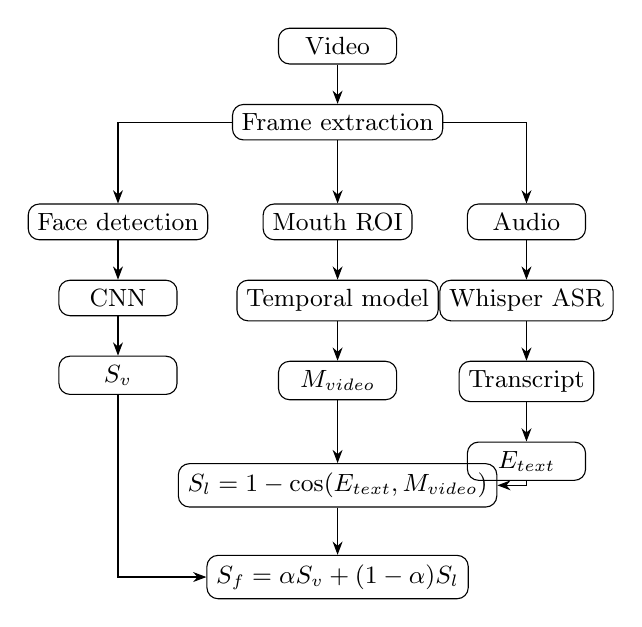
\begin{tikzpicture}[node distance=0.5cm and 0.6cm, box/.style={draw, rounded corners, minimum width=1.5cm, minimum height=0.45cm, font=\small}, arrow/.style={-Stealth}]

  \node[box] (video) {Video};
  \node[box, below=of video] (frames) {Frame extraction};
  \draw[arrow] (video) -- (frames);

  \node[box, below left=0.8cm and 0.3cm of frames] (face) {Face detection};
  \node[box, below=of face] (cnn) {CNN};
  \node[box, below=of cnn] (sv) {$S_v$};
  \draw[arrow] (frames) -| (face);
  \draw[arrow] (face) -- (cnn);
  \draw[arrow] (cnn) -- (sv);

  \node[box, below=0.8cm of frames] (mouth) {Mouth ROI};
  \node[box, below=of mouth] (temporal) {Temporal model};
  \node[box, below=of temporal] (mvid) {$M_{video}$};
  \draw[arrow] (frames) -- (mouth);
  \draw[arrow] (mouth) -- (temporal);
  \draw[arrow] (temporal) -- (mvid);

  \node[box, below right=0.8cm and 0.3cm of frames] (audio) {Audio};
  \node[box, below=of audio] (asr) {Whisper ASR};
  \node[box, below=of asr] (trans) {Transcript};
  \node[box, below=of trans] (etext) {$E_{text}$};
  \draw[arrow] (frames) -| (audio);
  \draw[arrow] (audio) -- (asr);
  \draw[arrow] (asr) -- (trans);
  \draw[arrow] (trans) -- (etext);

  \node[box, below=1.8cm of temporal] (sl) {$S_l = 1 - \cos(E_{text}, M_{video})$};
  \draw[arrow] (mvid) -- (sl);
  \draw[arrow] (etext) |- (sl);

  \node[box, below=0.6cm of sl] (sf) {$S_f = \alpha S_v + (1-\alpha) S_l$};
  \draw[arrow] (sv) |- (sf);
  \draw[arrow] (sl) -- (sf);
\end{tikzpicture}
\end{document}
